\newpage
МРНТИ 06.52.35
\hfill {\bfseries \href{https://doi.org/10.58805/kazutb.v.3.24-568}{https://doi.org/10.58805/kazutb.v.3.24-568}}

\sectionwithauthors{A.S. Baktymbet, S.S. Baktymbet, M.M. Idrisov, A. Serikkyzy}{INDUSTRIAL AND INNOVATIVE DEVELOPMENT: CHALLENGES AND PROSPECTS FOR KAZAKHSTAN (analytical review)}

\begin{center}
{\bfseries \textsuperscript{1}A.S. Baktymbet, \textsuperscript{2}S.S.
Baktymbet, \textsuperscript{3}M.M. Idrisov, \textsuperscript{4}A.
Serikkyzy\envelope}

\textsuperscript{1}Kazakh University of Technology and Business, Astana,
Kazakhstan,

\textsuperscript{2}Academy of Political Management, Astana, Kazakhstan,

\textsuperscript{3}Institute of Industrial Development, Almaty,
Kazakhstan,

\textsuperscript{4}ALMAU, Almaty, Kazakhstan
\end{center}

\envelope Corresponding author:
a.serikkyzy@almau.edu.kz

This paper explores the dynamics of industrial and innovative
development with a focus on Kazakhstan. It begins by examining the
principles guiding industrial and innovative strategies in foreign
countries, setting a comparative backdrop. The analysis then shifts to
Kazakhstan, detailing the major challenges confronting its manufacturing
industry, including structural inefficiencies and market constraints.
Further, the paper delves into the complexities and risks within
Kazakhstan\textquotesingle s oil and gas sector, highlighting both the
obstacles and potential growth areas. Finally, it assesses the prospects
and threats facing the country's mining and metallurgical complex,
offering insights into future trends and strategic recommendations. This
comprehensive review provides a nuanced understanding of
Kazakhstan\textquotesingle s industrial landscape and offers a framework
for navigating its evolving economic environment.

{\bfseries Key words:} industrial development, innovative strategies,
manufacturing challenges, economy growth, risks, prospects.

\sectionheading{РАЗВИТИЕ ПРОМЫШЛЕННОСТИ И ИННОВАЦИЙ: ВЫЗОВЫ И ПЕРСПЕКТИВЫ ДЛЯ КАЗАХСТАНА (аналитический обзор)}

\begin{center}
{\bfseries \textsuperscript{1}А.С. Бактымбет, \textsuperscript{2}С.С.
Бақтымбет, \textsuperscript{3}М.М. Идрисов, \textsuperscript{4}А. Серікқызы\envelope}

\textsuperscript{1}Казахский университет технологии и бизнеса им.
К.Кулажанова, г. Астана, Казахстан,

\textsuperscript{2}Академия политического менеджмента, г. Астана,
Казахстан,

\textsuperscript{3}Институт развития промышленности, г.Алматы,
Казахстан,

\textsuperscript{4}Университет ALMAU, Алматы, Казахстан,

e-mail: a.serikkyzy@almau.edu.kz
\end{center}

В данной статье рассматриваются динамика промышленного и инновационного
развития с акцентом на Казахстан. Сначала анализируются принципы,
руководствующие промышленными и инновационными стратегиями в зарубежных
странах, что создает сравнительный контекст. Затем внимание
переключается на Казахстан, где подробно рассматриваются основные
проблемы, с которыми сталкивается его производственный сектор, включая
структурные неэффективности и рыночные ограничения. В дальнейшем статья
исследует сложные вопросы и риски в нефтегазовом секторе Казахстана,
подчеркивая как препятствия, так и потенциальные области для роста.
Наконец, оцениваются перспективы и угрозы, с которыми сталкивается
горнодобывающий и металлургический комплекс страны, предлагаются
рекомендации по стратегии и прогнозирование будущих тенденций. Этот
всесторонний обзор предоставляет глубокое понимание промышленного
ландшафта Казахстана и предлагает основу для навигации в его
развивающейся экономической среде.

{\bfseries Ключевые слова:} промышленное развитие, инновационные стратегии,
проблемы производства, экономический рост, риски, перспективы.

\sectionheading{ӨНЕРКӘСІП ЖӘНЕ ИННОВАЦИЯНЫҢ ДАМУЫ: ҚАЗАҚСТАННЫҢ ҚАУІПТІЛЕРІ МЕН БОЛАШАҒЫ (аналитикалық шолу)}

\begin{center}
{\bfseries \textsuperscript{1}Ә.С. Бақтымбет, \textsuperscript{2}С.С.
Бақтымбет, \textsuperscript{3}М.М. Ыдырысов,
\textsuperscript{4}А. Серікқызы\envelope}

\textsuperscript{1}Қ.Құлажанов атындағы Қазақ технология және бизнес
университеті, Астана қ, Қазақстан,

\textsuperscript{2}Саяси менеджмент академиясы, Астана қ, Қазақстан,

\textsuperscript{3}Өнеркәсіптік даму институты, Алматы қ, Қазақстан,

\textsuperscript{4}Алматы менеджмент университеті, Алматы қ, Қазақстан,

e-mail: a.serikkyzy@almau.edu.kz
\end{center}

Бұл мақалада Қазақстанға баса назар аудара отырып, өнеркәсіптік және
инновациялық даму динамикасы қарастырылады. Алдымен шет елдердегі
өнеркәсіптік және инновациялық стратегияларды басқаратын принциптер
талданады, бұл салыстырмалы контекст жасайды. Содан кейін назар
Қазақстанға ауысады, онда құрылымдық тиімсіздіктер мен нарықтық
шектеулерді қоса алғанда, оның өндірістік секторының алдында тұрған
негізгі проблемалар егжей-тегжейлі қарастырылады. Одан әрі мақала
Қазақстанның мұнай-газ секторындағы күрделі мәселелер мен тәуекелдерді
зерттеп, кедергілерді де, өсу үшін әлеуетті салаларды да атап көрсетеді.
Ақырында, елдің тау-кен және металлургия кешенінің болашағы мен
қауіптері бағаланады, стратегия бойынша ұсыныстар және болашақ
тенденцияларды болжау ұсынылады. Бұл жан-жақты шолу Қазақстанның
өнеркәсіптік ландшафтын терең түсінуге мүмкіндік береді және оның дамып
келе жатқан экономикалық ортасында навигация үшін негіз ұсынады.

{\bfseries Түйін сөздер:} Өнеркәсіптік даму, инновациялық стратегиялар,
өндіріс проблемалары, экономикалық өсу, тәуекелдер,
перспективалар{\bfseries .}

\begin{multicols}{2}
{\bfseries Introduction}. The global landscape of industrial and innovative
development is continuously evolving, influenced by varying national
strategies and economic conditions. As nations adapt to shifting
technological advancements and market demands, understanding these
dynamics becomes crucial for assessing their own industrial policies and
growth trajectories. This paper provides an in-depth examination of
industrial and innovative development principles, contrasting them with
the unique challenges and opportunities faced by Kazakhstan.

Beginning with an overview of successful industrial strategies employed
by foreign states, the study sets the stage for a comparative analysis.
It then shifts focus to Kazakhstan, exploring the significant hurdles
encountered by its manufacturing sector, which include structural
inefficiencies and competitive pressures. The paper further investigates
the complex landscape of Kazakhstan's oil and gas industry, identifying
key risks and potential growth avenues. Additionally, it assesses the
prospects and existing threats within the mining and metallurgical
complex, offering a comprehensive view of the sector's evolving
landscape.

By integrating international perspectives with a detailed analysis of
Kazakhstan\textquotesingle s industrial environment, this paper aims to
provide valuable insights for policymakers, industry leaders, and
researchers interested in understanding and shaping Kazakhstan's
economic future.

{\bfseries Methods. Principles of industrial-innovative development in
foreign states.} If we look at international experience, we can identify
common principles and approaches for organizing and implementing state
policies in industrial-innovative development.

1. System of industrial-innovative development management.

Industrial countries generally have a similar organizational structure
for state management of industrial development. The main elements of
this structure are:

1) Clear legislative regulation of industrial policy, which allows for
centralized and balanced industrial policy throughout the country,
systematizes and focuses the process and conditions of state support for
industry.

2) A central government body responsible for industrial development
policy, related services, and their promotion in international markets
(its tasks include formulating industrial-innovative development policy
considering the state's strategic priorities, creating a comprehensive
system of incentives and support measures for industrial-innovative
projects and industrial clusters, conducting trade policy aimed at
creating opportunities for expanding existing and new productions).

3) A coordinated system of institutions supporting industrial-innovative
development, including industrial development funds or agencies.

4) Large state or national private companies, specifically designated by
the state, with powers to attract investments and implement large
industrial projects and establish production in new sectors.

5) A unified scientific, technological, and innovation policy, directed
by plans, strategies, and programs of sectoral ministries and agencies.

2. Focus on high-value-added exports rather than commodities.

The experience of countries (Ireland, Canada, Vietnam, Botswana, Saudi
Arabia, Morocco) that have successfully diversified their economies
shows that state support is often complemented by a comprehensive
export-oriented industrial policy, focused on high-value-added
manufacturing sectors and products, through investments in productivity,
human capital, transportation-logistics infrastructure, and technology
transfer.

In Ireland, the export growth of manufacturing products between 2010 and
2016 was 174 {[}1{]}. This was supported by a state policy focused on
business development. For instance, the country has established a
favorable tax regime and provides financial assistance for the creation
of companies and their entry into international markets.

Another example is Vietnam, where the government has introduced a new
economic development model since 2010, involving restructuring of
industry and services, with an emphasis on supporting the production of
high-tech goods {[}1{]}. This led to the formation of a favorable
investment regime, significantly increasing foreign direct investment
and creating 135 industrial and export zones {[}1{]}.

Canada has developed a state support system for exporters with key
elements including {[}2{]}:

- Consulting services for Canadian companies on research and target
market selection abroad (export preparation, market potential
assessment, network identification, and problem-solving).

- The MY TCS online platform -- access to market information and
business opportunities.

- The Can Export program -- financial support for a wide range of export
operations to increase the competitiveness of Canadian companies,
providing up to 50 million dollars over 5 years in direct financial
support for small and medium-sized exporters, funding companies from any
sector, covering 50\% of expenses.

- Financial support for business associations to create or expand
international cooperation.

- Business Women in International Trade -- providing targeted products
and services for women entrepreneurs aiming to enter global markets.

Canadian Technology Accelerators -- supporting high-growth Canadian
companies ready to enter global ICT and clean technology markets
{[}2{]}.

Thus, the key driver for export diversification is the private sector,
and states support their enterprises to develop and expand their export
capabilities through increased access to external markets beyond their
small domestic economies. In many countries, industrial growth is linked
to creating favorable conditions for access to large developed markets
(e.g., export subsidies, tax breaks, and easier financing).
High-value-added exports stimulate the production of quality goods,
work, and services, accelerates economic development, attracts foreign
capital into the manufacturing sector, and helps diversify revenue
sources in unstable global commodity markets.

3. International cooperation through integration into global value
chains.

Global value chains (GVCs) refer to the sequence of operations in which
products and services, undergoing various stages of development and
processing in different countries due to the global nature of the
economy, gain value (from the consumer's perspective).

Almost all countries aim to integrate into global value chains, which
enables technology transfer and enhances the country\textquotesingle s
industrial potential. However, developing countries must adhere to free
market rules -- offering the best quality at minimal cost {[}3{]}.

4. Development of value chains through attracting global players in
manufacturing sectors.

Transnational companies play a crucial role in global value chains. The
acceleration of globalization and the worldwide distribution of
available raw materials, cheap labor, and potential markets have led
transnational companies to benefit from maintaining geographically
separated production facilities, research and development centers, and
markets. The primary value is created not in the physical production of
goods but in high-tech areas with a concentration of highly qualified
labor.

Conversely, concentrating highly qualified specialists, scientific
infrastructure, and engineering systems in manufacturing industries
allows countries to increase competencies in advancing in the value
chain, moving from lower to middle and upper-tier production. The main
distinctions of these product categories are the complexity of the
produced goods and their dependence on primary raw materials.

Lower-tier products typically use primary raw materials directly, whose
prices are often set on commodity exchanges and are fluctuating, leading
to variability in production volume and export depending on external
conditions. On the other hand, middle and upper-tier products have more
stable production and are less dependent on primary raw material prices,
as high technology and scientific labor constitute a larger portion of
their cost.

Therefore, developing countries focus on creating attractive offers for
transnational companies, balanced by the "price/quality" criterion. Key
aspects of integrating into global value chains include developing a
strong scientific-technological base, building a qualified workforce,
effectively using opportunities within international integration
associations, developing trade agreements with promising partners, and
implementing cluster policies to enhance value chains and
competitiveness within the country.

In Kazakhstan, further integration into global value chains is
necessary, with an expansion of cooperation with existing and new
transnational companies. Developing relationships with transnational
companies already operating in Kazakhstan should be based on mutually
beneficial cooperation considering Kazakhstan\textquotesingle s
interests. This will be achieved through expanding the range of produced
goods and deepening production to diversify and complicate the
country\textquotesingle s economy.

It should be noted that several global transnational companies (e.g.,
Arcelor Mittal, POSCO, LOTTE, Schneider Electric) are currently
operating in the country {[}1{]}. However, these companies are either
working with Kazakh enterprises in lower-tier production, outdated
products, or have just begun fruitful cooperation. Therefore, a balanced
and planned approach to cooperation with transnational companies is
needed to develop and deepen existing cooperation. A notable example of
integration into global value chains in Kazakhstan is the limited
liability partnership "POSUK Titanium," which produces titanium slabs
that are subsequently supplied to Boeing through the value chain
{[}1{]}.

Attracting new transnational companies should also align with the
state\textquotesingle s interests in achieving set goals, specifically
producing new high-value-added goods and exporting to global markets
through the distribution channels of transnational partners.

5. Implementing tools for attracting global players to integrate into
global value chains.

One of the primary tasks for attracting foreign investors should be
focusing on global leaders in manufacturing industries that have their
distribution channels in the global value chain.

Investment planning and integration into global value chains will
include implementing a unified map of priority goods and services. This
tool involves identifying a list of the most promising goods/product
groups for localization within the country, considering workforce,
technological, and raw material availability, as well as export markets.

This list of goods addresses both state and business interests. From the
state's perspective, priority goods will focus on expanding product
range, diversification, and complexity of production. For businesses,
the list can serve as a guide for creating new productions with growth
potential and entry into external markets.
\end{multicols}

\begin{figure}[H]
	\centering
	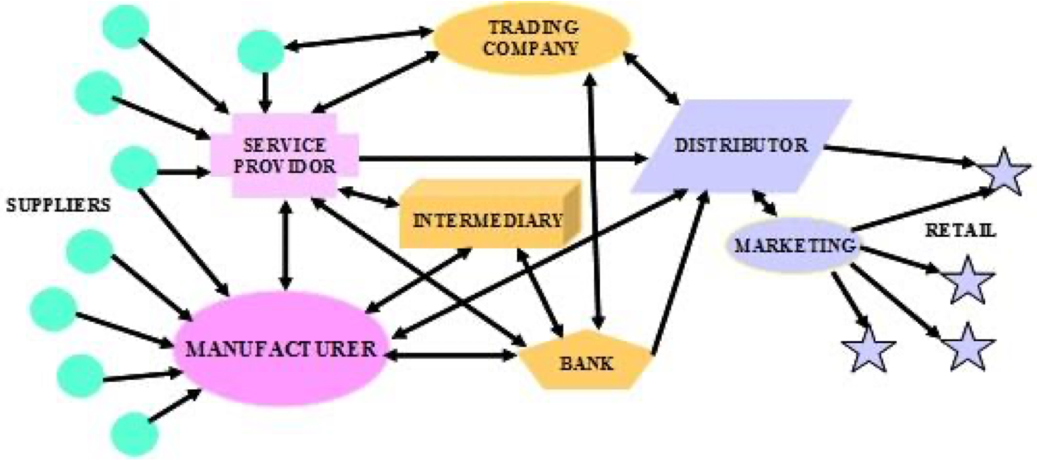
\includegraphics[width=0.6\textwidth]{assets/340}
	\caption*{Figure 1 - Global value chains, commodity chains and production networks {[}3{]}.}
\end{figure}

\begin{multicols}{2}
6. Development of new production types for value addition in the market
and export.

The use of rare and rare-earth metals is crucial in complex industries
such as electronics, medicine, and computer manufacturing. The
development of finished products from these metals reflects the
technological advancement of the industry.

Currently, global demand for rare-earth elements is around 120,000 tons
per year {[}4{]}. However, the global market for rare-earth metals is
almost monopolized by Chinese production. Supply restrictions are
negatively impacting other countries\textquotesingle{} industries.
Consequently, major economies actively using rare-earth metals (USA,
Russia, Japan, Germany) are planning to reduce their dependency on
Chinese supplies. An example of this shift is the agreement between the
United States and Australia for joint mining and processing of minerals,
including rare-earth metals {[}5{]}.

Constant technological progress increases global demand for rare-earth
metal products. Moreover, upper-tier products, which involve high value
addition and technological complexity, are also significant.

Kazakhstan has substantial reserves and prospects for expanding its
mineral resource base of rare and rare-earth metals. The
republic\textquotesingle s production of these metals is carried out at
specialized enterprises.

Currently, the industry urgently needs investments, primarily for
improving infrastructure in mining regions. With effective use of rare
and rare-earth minerals, Kazakhstan can develop modern science and
technology sectors and market these metals globally.

{\bfseries Results}. {\bfseries Trends and challenges in Kazakhstan's
manufacturing industry.}

In 2022, the manufacturing sector\textquotesingle s output totaled 21.2
trillion tenge. The main contributors to the manufacturing industry are
metallurgy (44\% of the total sector), food production (19\%), machine
engineering (15\%), construction materials production (6\%), and
chemical industry (4\%) {[}6{]}.

Manufacturing accounts for 13.4\% of the country\textquotesingle s GDP.
In this regard, Kazakhstan remains a net importer for all categories of
goods except metallurgy. The highest net imports are observed in machine
engineering (7.6 trillion tenge), the chemical industry (1.4 trillion
tenge), and food production (0.9 trillion tenge) {[}6{]}.

The observed underutilization of production capacities indicates a low
level of competitiveness among domestic manufacturers: 70\% of
manufacturing enterprises have an average annual capacity utilization
rate of no more than 70\%, and the average annual capacity utilization
rate in the machine engineering sector has fluctuated between 25\% and
48\% in recent years. {[}6{]}.

{\bfseries Key challenges facing Kazakhstan's manufacturing industry.}

1. Low complexity of produced goods.

- Despite overall sector development, the share of raw materials in
exports remains at 66\%, while the proportion of local manufacturing
enterprises engaged in innovative activities is only 14.8\%.
Consequently, Kazakhstan has a negative economic complexity index
(-0.47) and ranks 88th out of 133 countries in this indicator, trailing
behind neighboring countries with similar economies (Russia - 53rd place
(0.19), Turkey - 40th place (0.61), and Belarus - 29th place (0.91))
{[}7{]}.

- In Kazakhstan, the depth of processing in raw material sectors is low,
with most products being exported as intermediate raw materials. For
example, 77\% of lead, 87\% of aluminum, and 99\% of copper are exported
in an unprocessed or minimally processed state {[}8{]}.

- Despite having a raw material base, Kazakhstan has not developed a
significant gas or petrochemical sector, and only in 2022 was the first
large-scale gas chemical project launched. Raw materials from Tengiz,
Kashagan, and Karachaganak contain high levels of fatty gas fractions
(ethane, propane, butane) necessary for gas chemical production.
Currently, fatty fractions are only extracted from raw materials from
the Tengiz field, which supplies polypropylene production (KPI) {[}8{]}.

Additionally, existing enterprises face raw material unavailability and
shortages: the volume of imported raw materials and components for the
manufacturing sector exceeds 50\%, which increases production costs and
creates barriers to establishing high-tech manufacturing. For instance,
imports constitute a significant portion of raw materials and components
for industrial equipment, vehicles, and agricultural machinery, while
the main output in machine engineering comprises simple assembly
operations with minimal localization.

- The insufficient level of international technology and standard
implementation in production is another factor reducing the economic
complexity index. This process requires technological upgrades and
substantial investments, which, in turn, affects the competitiveness of
domestic products.

2. Wear and low energy efficiency of production.

- The average level of wear is 41\%, with higher levels in the
production of metal products, beverages, weapons, military equipment,
and other machine engineering products exceeding 45\% {[}8{]}.

- Energy costs in Kazakhstan\textquotesingle s mining and metallurgical
complex are among the highest in the world. With energy intensity at 1.6
tons of oil equivalent per thousand USD, Kazakhstan\textquotesingle s
products lag significantly behind developing and developed markets,
where this figure ranges from 0.2 to 0.9 tons of oil equivalent per
thousand USD {[}8{]}.

{\bfseries Discussion}. {\bfseries Problems, risks, and opportunities in
Kazakhstan\textquotesingle s oil and gas sector.} Oil and gas production
continues to have a significant impact on Kazakhstan\textquotesingle s
economy: in 2022, the sector\textquotesingle s gross added value (GAV)
amounted to 11\% of GDP, with the sector\textquotesingle s share in
total goods exports exceeding 50\%, and in net investment inflow --
almost 40\% {[}8{]}.

Annually, oil production prospects in Kazakhstan fall short of
expectations. According to the current forecast, considering the
modernization of production at major fields, peak production is expected
to reach 104 million tons by 2030. Among the existing major fields, the
most significant decline in production is anticipated at Kashagan: in
2021, its expected peak production volume was reduced by 40\% compared
to the 2017 forecast {[}8{]}.

Additionally, one of the challenges is the depletion of deposits. For
instance, according to international experts\textquotesingle{}
forecasts, several major companies within KazMunayGas are expected to
see a 15-30\% decline in production by 2030. In this context,
sustainable reduction in production and the closure of depleting fields
are critical both from environmental and social perspectives. Moreover,
in the medium term, there is a risk of a shortage of oil raw materials
in addition to the expected gas deficit in 2024-2025, as local demand is
met by the KazMunayGas fields {[}8{]}.

International experts note that from 2017 to 2022, the forecast for
production at fields in the development and exploration stages also
dropped from 65 to 6 million tons {[}8{]}. The attractiveness of
exploring and developing new fields is limited by the pricing of raw
material supplies to the domestic market.

In addition to resource base constraints, the risk of raw material
shortages is exacerbated by the rapid growth in fuel consumption in
Kazakhstan. Per capita diesel fuel consumption (about 30\% of the demand
for petroleum products) significantly exceeds that of neighboring
countries. Moreover, fuel prices in Kazakhstan are among the lowest in
the region and the world, and the creation of common oil, gas, and
petroleum product markets within the EAEU in 2025 could lead to a flow
of lubricants to neighboring countries, further reducing domestic fuel
availability. According to the analytical company IHS Markit, if the
current consumption trajectory remains, by 2025, the demand for
petroleum products will reach 19 million tons of refined oil and exceed
the capacities of oil refineries {[}8{]}.

There are several opportunities for developing additional supply
corridors through the Trans-Caspian and Chinese routes. Current oil
transshipment through the Aktau port is 2.2 million tons per year with
the port\textquotesingle s technical capacity at 7 million tons per year
(available volume - 4.8 million tons). The Atasu - Alashankou pipeline
handles about 11 million tons per year, including 10 million tons of
transit. The technical capacity of this pipeline is approximately 17.5
million tons per year (available volume - 6.5 million tons) {[}8{]}.

In the gas transportation system, existing constraints mainly concern
transportation for domestic consumption. There is significant wear and
load on several key infrastructure facilities, such as the Beineu -
Bozoy - Shymkent pipeline and underground gas storage facilities.

{\bfseries Prospects and threats for Kazakhstan's mining and metallurgical
complex.}

Kazakhstan\textquotesingle s mining and metallurgical complex (MMC) is
one of the key drivers of the country\textquotesingle s economic growth:
in 2022, the total gross added value (GAV) from metal mining, coal,
lignite, and other solid minerals (SMs), as well as the metallurgical
industry, reached nearly 10\% of the economy, and over 25\% in exports.

However, the MMC faces key challenges and opportunities that will
determine its future development.

Kazakhstan is experiencing low levels of reserves prepared for
development, insufficient replenishment of reserves, a decline in
average ore content and increased complexity in processing ore bodies.
The availability of prepared copper reserves is 10-12 years; chromite
reserves suitable for open-pit mining have been depleted; the
availability of proven iron ore reserves suitable for open-pit mining is
20-25 years.

A critical factor affecting the situation is the low activity in
geological exploration. The legal reform in the mineral resource sector
has drastically changed its regulatory framework, providing more
competitive access to subsoil resources.

Currently, only 16\% of the country\textquotesingle s territory
available for exploration has been licensed. In 2022, the unit costs for
geological exploration in Kazakhstan were only \$63 per km², which is
significantly lower than the global average (\$88 per km² for metals)
and the figures for leading mining countries such as the USA, Canada,
and Australia (\$170 - \$300 per km²) {[}8{]}.

In addition to the insufficient replenishment of existing reserves, the
country has significant unrealized potential in the most rapidly growing
and promising metals used in modern batteries and electronics: nickel,
cobalt, and lithium. Another rapidly growing and unrealized category in
Kazakhstan is rare earth metals.

Another challenge for the sector is the rising cost of labor. Since
2000, the average cost per employee in the MMC has increased sevenfold,
reaching \$1,190 per month. However, wage increases have not been
accompanied by a comparable rise in labor productivity in the sector,
which remains at a relatively low level: in 2020, labor productivity in
Kazakhstan was \$62,000 per employee per year, compared to \$114,000 in
Peru and \$160,000 - \$200,000 in developed countries (Norway,
Australia, Canada, Ireland, Sweden) {[}8{]}.

Transportation and logistics constraints, such as the distance from key
markets, resulting in complex and costly logistics, as well as risks
related to the limited export transportation corridors, negatively
impact the competitiveness of Kazakhstan\textquotesingle s MMC products.

{\bfseries Conclusion.} In conclusion, the interplay between industrial and
innovative development strategies is pivotal in shaping the economic
future of nations. This paper has provided a comparative overview of
global industrial practices and analyzed the specific challenges and
opportunities faced by Kazakhstan. The examination of
Kazakhstan\textquotesingle s manufacturing sector reveals critical
inefficiencies and competitive constraints that require targeted reforms
and strategic investments. Similarly, the analysis of the oil and gas
sector highlights both significant risks and promising growth
opportunities that must be carefully managed to ensure sustainable
development.

The insights into Kazakhstan's mining and metallurgical complex
underscore the need for a balanced approach to harness its potential
while mitigating associated threats. By integrating international best
practices with a thorough understanding of local contexts, Kazakhstan
can better navigate its industrial and economic challenges.

Ultimately, the path forward for Kazakhstan involves leveraging its
existing strengths, addressing critical vulnerabilities, and adopting
innovative strategies to foster long-term growth and stability. This
comprehensive analysis serves as a foundational guide for policymakers,
industry stakeholders, and researchers dedicated to advancing
Kazakhstan's industrial capabilities and economic resilience.

\emph{{\bfseries Financing}. This work was financially supported by the
Science Committee of the Ministry of Science and Higher Education of the
Republic of Kazakhstan (grant AP1968020, 2023--2025).}
\end{multicols}

\begin{center}
{\bfseries References}
\end{center}


\begin{noparindent}
1.
The Government of the Republic of Kazakhstan (2019). State Program for
Industrial-Innovative

Development of the Republic of Kazakhstan for
2020-2025. URL:

https://adilet.zan.kz/rus/docs/P1900001050 (date of
application - 16.09.2024)

2.
Grigorieva E. Supporting the Export of Agricultural Products in
Canada. -2016. URL:

https://cyberleninka.ru/article/n/sodeystvie-eksportu-produktsii-apk-v-kanade

(date of application - 16.09.2024)

3.
Todeva E., Rakhmatullin R. Industry Global Value Chains, Connectivity
and Regional Smart Specialisation in Europe. -2016. --URL:
http://www.bcned.co.uk/images/reports/research/JRC102801\_lfna28086enn.pdf
(date of application - 16.09.2024)

4.
Metal Mining The Rare Earth Metals: From Strength to Compactness.
-2017. URL:

https://metalmininginfo.kz/archives/4688 (date of
application - 16.09.2024)

5.
Prokhorov I. The Rare Earth Metals Market Shows Steady Growth. -2017.
URL:

https://www.gmprom.kz/analytics/rynok-redkozemelnyh-metallov-pokazyvaet-ustojchivyj-rost/

(date of application - 16.09.2024)

6.
Ministry of industry and construction of the Republic of Kazakhstan
Growth in Kazakhstan\textquotesingle s manufacturing industry reached
4.1\%. -2024. URL:

https://www.gov.kz/memleket/entities/mps/press/news/details/727688?lang=en

(date of application - 16.09.2024)

7.
Karimov E. Economic Complexity Index: India and Kazakhstan. -2024.
URL: https://economy.kz/?p=5210 (date of application - 16.09.2024)

8.
The Government of the Republic of Kazakhstan The National Development
Plan of the Republic of Kazakhstan until 2029. -2024. URL:
https://adilet.zan.kz/rus/docs/U2400000611 (date of application -
16.09.2024)
\end{noparindent}

\emph{{\bfseries Information about authors}}

\begin{noparindent}
Baktymbet A.S. - c.e.s., assistant professor at the Kazakh University of
Technology and Business, Astana, Kazakhstan, e-mail:
asembaktymbet@gmail.com;

Baktymbet S.S.-c.e.s, assistant professor, Academy of Political
Management, Astana, Kazakhstan, e-mail: saule\_sbs@mail.ru;

Idrisov M.M. - Director of the Institute of Industrial Development,
Almaty, Kazakhstan, e-mail:

m.idrissov.kz@gmail.com;

Serikkyzy A .- PhD, associate professor ALMAU, Almaty, Kazakhstan,
e-mail:

a.serikkyzy@almau.edu.kz
\end{noparindent}

\emph{{\bfseries Сведения об авторах}}

\begin{noparindent}
Бактымбет Ә.С. - к.э.н., доцент Казахского университета технологий и
бизнеса, Астана, Казахстан

e-mail: asembaktymbet@gmail.com;

Бақтымбет С.С. -- к.э.н., доцент, Академия политического менеджмента,
Астана, Казахстан, e-mail: saule\_sbs@mail.ru;

Идрисов М. М. -- директор Института промышленного развития, Алматы,
Казахстан email:

m.idrissov.kz@gmail.com;

Серіккызы А. - PhD, ассоциированный профессор ALMAU, Алматы, Казахстан,
e-mail:

a.serikkyzy@almau.edu.kz
\end{noparindent}
